\begin{figure}[ht!]
    \begin{subfigure}{.45\textwidth}
    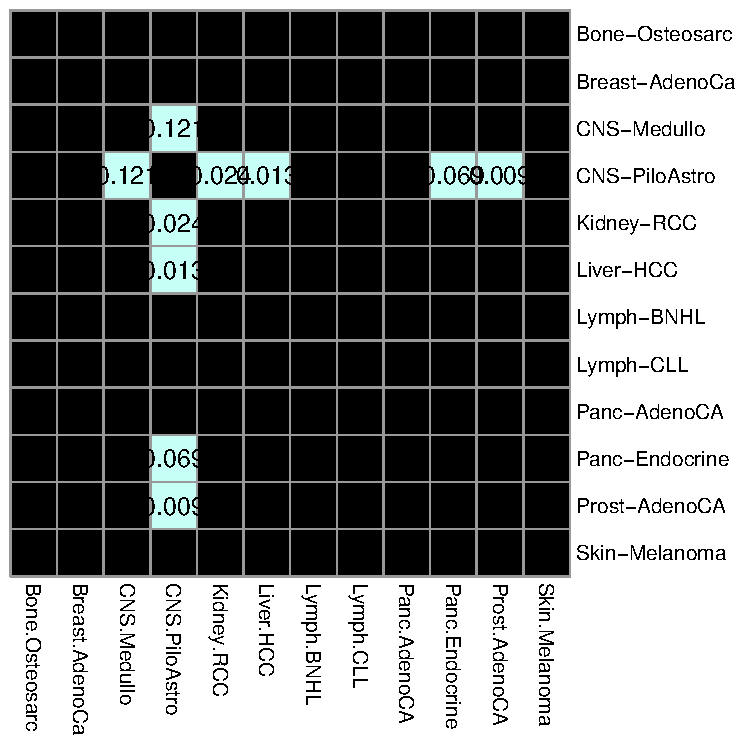
\includegraphics[scale=0.65]{graphics/bootstrap_bins_euclidean.pdf}
    \caption{Bins/Euclidean}
    \label{fig:bootstrap_bins_euclidean}
    \end{subfigure}
    ~
    \begin{subfigure}{.55\textwidth}
    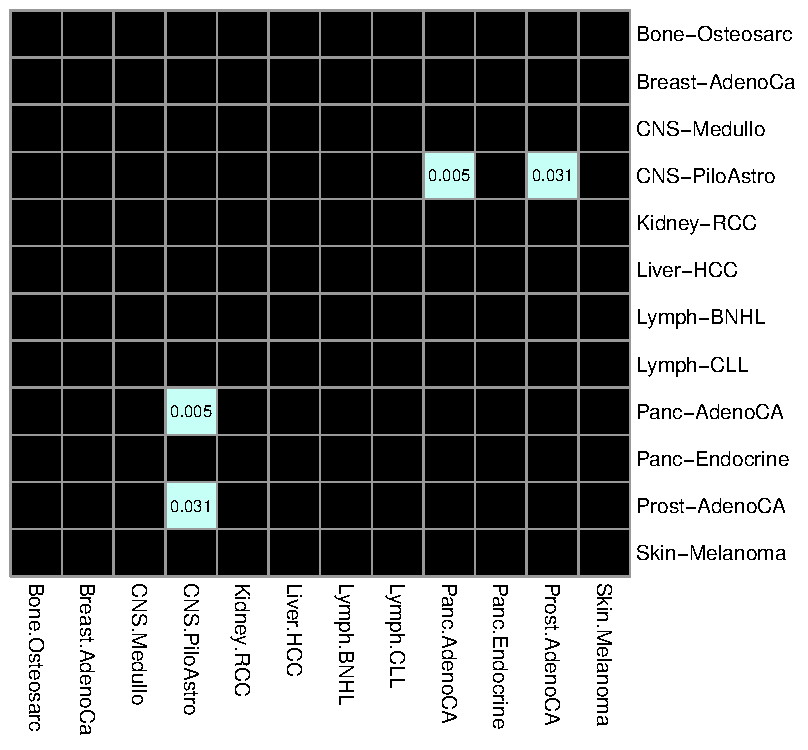
\includegraphics[scale=0.65]{graphics/bootstrap_bins_wasserstein.pdf}
    \caption{Bins/Wasserstein}
    \label{fig:bootstrap_bins_wasserstein}
    \end{subfigure} \\
    \vspace{0.5cm}
    
    \begin{subfigure}{.45\textwidth}
    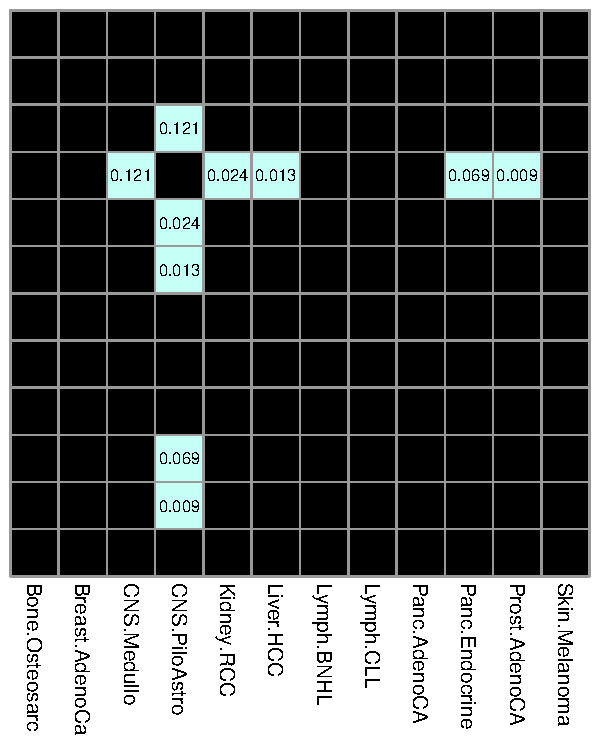
\includegraphics[scale=0.65]{graphics/bootstrap_smooth_euclidean.pdf}
    \caption{Smooth/Euclidean}
    \label{fig:bootstrap_smooth_euclidean}
    \end{subfigure}
    ~
    \begin{subfigure}{.55\textwidth}
    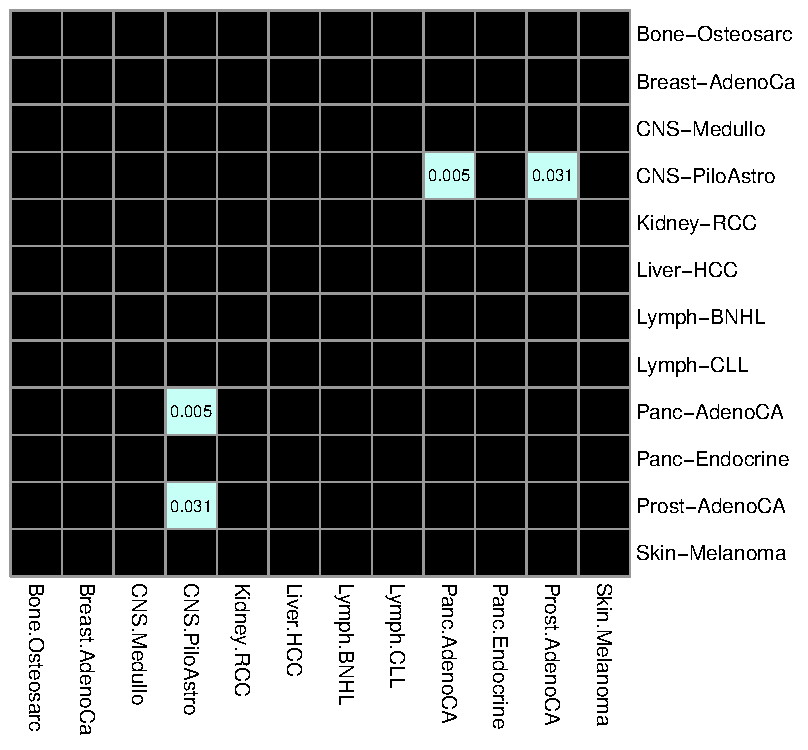
\includegraphics[scale=0.65]{graphics/bootstrap_smooth_wasserstein.pdf}
    \caption{Smooth/Wasserstein}
    \label{fig:smooth_wasserstein}
    \end{subfigure} \\
    \caption{\textbf{GLE was generally significantly different between cancers according to bootstrap hypothesis test using (a) Bin/Euclidean, (b) Bin/Wasserstein, (c) Smooth/Euclidean, (d) Smooth/Wasserstein.} The row labels in (a) and (c) are the same as (b) and(d). No multiple test correction was applied. For all four panels, black cells represent p-values $<0.001$, coloured cells are annotated with the p-values, the p-values on the diagonals compare a cancer to itself and should always be 1. The p-value matrices are symmetric.}
    \label{fig:gle_bootstrap}
\end{figure}